\documentclass[final]{beamer}

\usepackage[scale=1.2, width=56in, height=42in]{beamerposter} % Use the beamerposter package for laying out the poster
\usepackage{epstopdf}
\usepackage{tipa}
\usepackage{booktabs}
\DeclareFontSubstitution{T3}{ptm}{m}{n}
\usetheme{confposter} % Use the confposter theme supplied with this template
\setbeamercolor{block title}{fg=ddblue,bg=white} % Colors of the block titles
\setbeamercolor{block body}{fg=black,bg=white} % Colors of the body of blocks
\setbeamercolor{block alerted title}{fg=white,bg=dblue!70} % Colors of the highlighted block titles
\setbeamercolor{block alerted body}{fg=black,bg=dblue!10} % Colors of the body of highlighted blocks
\setbeamertemplate{itemize items}[circle]
% Many more colors are available for use in beamerthemeconfposter.sty

%-----------------------------------------------------------
% Define the column widths and overall poster size
% To set effective sepwid, onecolwid and twocolwid values, first choose how many columns you want and how much separation you want between columns
% In this template, the separation width chosen is 0.024 of the paper width and a 4-column layout
% onecolwid should therefore be (1-(# of columns+1)*sepwid)/# of columns e.g. (1-(4+1)*0.024)/4 = 0.22
% Set twocolwid to be (2*onecolwid)+sepwid = 0.464
% Set threecolwid to be (3*onecolwid)+2*sepwid = 0.708

\newlength{\sepwid}
\newlength{\onecolwid}
\newlength{\twocolwid}
\newlength{\threecolwid}
\setlength{\paperwidth}{56in} % A0 width: 46.8in
\setlength{\paperheight}{42in} % A0 height: 33.1in
\setlength{\sepwid}{0.02\paperwidth} % Separation width (white space) between columns
\setlength{\onecolwid}{0.18\paperwidth} % Width of one column
\setlength{\twocolwid}{0.54\paperwidth} % Width of two columns
\setlength{\threecolwid}{0.708\paperwidth} % Width of three columns
\setlength{\topmargin}{-0.5in} % Reduce the top margin size
%-----------------------------------------------------------

\usepackage{graphicx}  % Required for including images
\usepackage{booktabs} % Top and bottom rules for tables

%-------------------------------------------------------------------------------------
%	TITLE SECTION 
%-------------------------------------------------------------------------------------

\title{Source properties of dorsal fricatives} % Poster title

\author{Charles Redmon and Allard Jongman}
\institute{Department of Linguistics, University of Kansas} % Institution(s)

%----------------------------------------------------------------------------

\setbeamertemplate{headline}{
 \leavevmode
  \begin{columns}
   \begin{column}{.2\linewidth}
    
\includegraphics[height=7cm]{KUlogo.eps}
   \end{column}
   \begin{column}{.6\linewidth}
    \vskip1cm
    \centering
    \usebeamercolor{title in headline}{\color{jblue}\Huge{\inserttitle}\\[1ex]}
    \usebeamercolor{author in headline}{\color{fg}\large{\insertauthor}\\[1ex]}
    \usebeamercolor{institute in headline}{\color{fg}\normalsize{\insertinstitute}\\[1ex]}
    \normalsize{The 5th Joint Meeting of the Acoustical Society of America and the Acoustical Society of Japan: Honolulu, 2016}
    \vskip1cm
   \end{column}
   \begin{column}{.2\linewidth}
    \hspace{4cm}
    \includegraphics[height=7cm]{asjLogo.png}
    \hspace{3cm}
    \includegraphics[height=7cm]{asaLogo.png}
   \end{column}
   \vspace{1cm}
  \end{columns}
 \vspace{0.5in}
 \hspace{1in}\begin{beamercolorbox}[wd=54in,colsep=0.15cm]{cboxb}\end{beamercolorbox}
 \vspace{0.1in}
}

%----------------------------------------------------------------------------------------

\begin{document}

\addtobeamertemplate{block end}{}{\vspace*{2ex}} % White space under blocks
\addtobeamertemplate{block alerted end}{}{\vspace*{2ex}} % White space under highlighted (alert) blocks

\setlength{\belowcaptionskip}{2ex} % White space under figures
\setlength\belowdisplayshortskip{2ex} % White space under equations

\begin{frame}[t] % The whole poster is enclosed in one beamer frame

\begin{columns}[t] % The whole poster consists of three major columns, the second of which is split into two columns twice - the [t] option aligns each column's content to the top

\begin{column}{\sepwid}\end{column} % Empty spacer column

\begin{column}{\onecolwid} % The first column

%------------------------------------------------
%	OBJECTIVES
%------------------------------------------------

\begin{block}{Background}
  \begin{itemize}
    \item Models of voiceless fricative acoustics rely on the assumption that the sound source at the supralaryngeal constriction is aperiodic\textsuperscript{\color{blue} 1} 
      \begin{itemize}
        \item This simplifying assumption accounts for a wide range of fricative places of articulation\textsuperscript{\color{blue} 1--6}
      \end{itemize}
    \item However, for voiceless \textbf{velar} \textipa{/x/} and \textbf{uvular} \textipa{/X/} fricatives (jointly referred to as \textbf{dorsal fricatives, X}) the potential for high-velocity airflow to induce vibration of the uvula means such sounds may in some instances be excited by a \textbf{mixed source}
      \begin{itemize}
        \item Data from previous studies support this expectation\textsuperscript{\color{blue} 1,7--11}
      \end{itemize}
  \end{itemize}
\end{block}

%References:
% 1. Fant (1960)
% 2. Stevens (1971)
% 3. Shadle (1985)
% 4. Alwan (1986)
% 5. Narayanan and Alwan (2000)
% 6. Jongman et al. (2000)
% 7. Zeroual (2003)
% 8. Jesus and Shadle (2005)
% 9. Shosted & Chikovani (2006)
% 10. Shosted (2008)
% 11. Yeou and Maeda (2011)


%------------------------------------------------

\begin{block}{Research Questions}
\begin{itemize}
     \item How common are mixed-source productions of voiceless dorsal fricatives and what is their relative positional and vocalic distribution?
     \item What are the acoustic consequences of uvular vibration when present?
\end{itemize}
\end{block}

%------------------------------------------------

\begin{block}{Participants}
  \begin{itemize}
    \item 4 native speakers (2F) each of Arabic, Persian, and Spanish
    \item All 12 participants grew up in Saudi Arabia, Iran, or Spain, respectively
  \end{itemize}
\end{block}

%------------------------------------------------

\begin{block}{Materials}
  \begin{itemize}
     \item 2 fricatives /s, X/ in 3 vowel contexts /i, a, u/ in 2 positions (CV, VC) formed the target set 
     \item 3 words containing each target sequence were recorded in sentence frames in 4 repetitions
     \item The same list was recorded twice:
       \begin{enumerate}
         \item Acoustic data was recorded with a head-mounted microphone in an anechoic chamber 
         \item Oral and nasal airflow was recorded with the Scicon R\&D (2015) system
       \end{enumerate}
     \item Acoustic signals were digitized at 22.05 kHz, and airflow signals were digitized at 11 kHz and low-pass filtered at 200 Hz
  \end{itemize}
\end{block}

%------------------------------------------------

\begin{block}{Source Estimation}
  \begin{itemize}
    \item Frequency of oscillation in airflow was estimated through the power spectral density (PSD) of the autocorrelation function $R(\tau)$ over 60 ms windows sampled in 10 ms steps
    \item Reference pitch floors by speaker were used to ensure any periodicity was not due to voicing
  \end{itemize}
  \vspace{0.25in}
  \begin{figure}
    \includegraphics[width=\linewidth]{plots/measurement1.pdf}
    \caption{Measurement illustration and definitions.}
  \end{figure}
\end{block}

\end{column}

%------------------------------------------------
%------------------------------------------------

\begin{column}{\sepwid}\end{column} % Empty spacer column

\begin{column}{\twocolwid} % Begin a column which is two columns wide (column 2)

\begin{block}{Aerodynamic Data}

\begin{columns}[t,totalwidth=\twocolwid] % Split up the two columns wide column

\begin{column}{0.31\twocolwid} % The first column within column 2 (column 2.1)

\begin{figure}
\includegraphics[width=0.85\linewidth]{plots/arabicSignal.pdf}
\caption{Sample production of the Arabic word /Xa\textlengthmark ru\textlengthmark f/ by speaker AM02. The estimated oscillation frequency in this token is 61.8 Hz.}
\end{figure}

\end{column}

\begin{column}{0.31\twocolwid} % The first column within column 2 (column 2.1)

\begin{figure}
\includegraphics[width=0.85\linewidth]{plots/persianSignal1.pdf}
\caption{Sample production of the Persian word /Xa\textlengthmark k/ by speaker PF02. The estimated oscillation frequency in this token is 93.5 Hz.}
\end{figure}

\end{column}

\begin{column}{0.31\twocolwid} % The first column within column 2 (column 2.1)

\begin{figure}
\includegraphics[width=0.85\linewidth]{plots/spanishSignal.pdf}
\caption{Sample production of the Spanish word /Xade/ by speaker SF01. The estimated oscillation frequency in this token is 77.4 Hz.}
\end{figure}

\end{column}

\end{columns} % End of the split of column 2 - any content after this will now take up 2 columns width


%--------------------------------------------------
\begin{column}{\sepwid}\end{column} % Empty spacer column
%--------------------------------------------------


\begin{columns}[t,totalwidth=\twocolwid] % Split up the two columns wide column again

\begin{column}{0.315\twocolwid} % 1/4 column

\begin{figure}
\includegraphics[width=\linewidth]{plots/distPlot.pdf}
\caption{Distribution of mixed-source /X/ tokens by Language, Position, and Vowel. Speaker IDs are truncated (e.g. M01 for PM01) for space.}
\end{figure}

\end{column} % End of column 2.1

\begin{column}{0.315\twocolwid} % The first column within column 2 (column 2.1)

\begin{figure}
\includegraphics[width=\linewidth]{plots/frequency.pdf}
\caption{Estimated frequencies of oscillation by Language, Position, and Vowel Context. Error bars represent $\pm$ 1 standard error.}
\end{figure}

\end{column} % End of column 2.1

\begin{column}{0.315\twocolwid} % The first column within column 2 (column 2.1)

  \begin{figure}
    \includegraphics[width=\linewidth]{plots/jitter.pdf}
    \caption{Relative Jitter in the base frequency of a representative sample ($n$ = 148) of mixed-source tokens across Language, Position, and Vowel.}
  \end{figure}

\end{column} % End of column 2.1

\end{columns} % End of the split of column 2


\begin{columns}[t,totalwidth=\twocolwid] % Split up the two columns wide column again

\begin{column}{0.49\twocolwid} % 1/4 column

\begin{itemize}
  \item Arabic and Persian, relative to Spanish, show more consistent productions of the dorsal fricative with some degree of uvular vibration
  \item Oscillation frequency in word-initial position is reliably lower in the context of the high front vowel \textipa{/i/} than before the low back vowel \textipa{/a/}
\end{itemize}

\end{column}

\begin{column}{0.49\twocolwid} % 1/4 column
  \begin{itemize}
    \item Oscillation frequency is much less stable (higher percentage jitter) than would be expected for voiced fricatives or trills, which is consistent with the characterization of the process as a random vibration. No clear patterns emerged in Position or Vowel Context comparisons across languages, however.
  \end{itemize}
\end{column}

\end{columns}

\end{block}



\begin{block}{Acoustic Data}

\begin{columns}[t,totalwidth=\twocolwid] % Split up the two columns wide column again

\begin{column}{0.32\twocolwid} % 1/4 column

  \begin{figure}
    \includegraphics[width=\linewidth]{plots/xuTbaSpectra.pdf}
    \caption{Spectra from the middle 60 ms of /X/ in two repetitions of the word /Xut\textsuperscript{\textrevglotstop}ba/ produced by speaker AF02, one with uvular vibration (red) and one without (blue). An index of the presence of vibration, $A_s$--$A_f$, the source component amplitude minus the filter component (spectral peak) amplitude, is shown with the solid and dashed arrows, respectively. In Figures \ref{fig:peak} and \ref{fig:mean} we have used this measure to classify dorsal fricative tokens (Acc.: 98\%, Spec.: 100\%) into Aperiodic and Mixed source types.}
  \end{figure}

\end{column} % End of column 2.1

\begin{column}{0.3\twocolwid} % The first column within column 2 (column 2.1)

  \begin{figure}
    \includegraphics[width=\linewidth]{plots/spectralPeak.pdf}
    \caption{Spectral peak frequencies by source type.}
    \label{fig:peak}
  \end{figure}

\end{column} % End of column 2.1

\begin{column}{0.3\twocolwid} % The first column within column 2 (column 2.1)

  \begin{figure}
    \includegraphics[width=\linewidth]{plots/spectralMean.pdf}
    \caption{Spectral means by source type.}
    \label{fig:mean}
  \end{figure}

\end{column}

\end{columns}



\end{block}

\end{column} % End of the second column

\begin{column}{\sepwid}\end{column} % Empty spacer column

\begin{column}{\onecolwid} % The third column

%----------------------------------
%	CONCLUSION
%----------------------------------

\begin{block}{Synthesis}

  \begin{figure}
    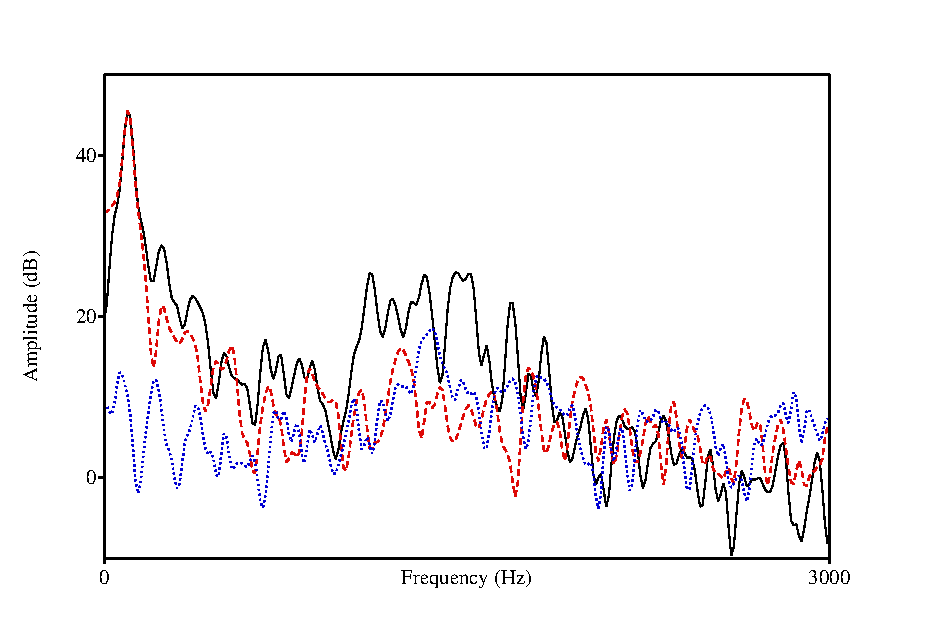
\includegraphics[width=\linewidth]{plots/synthPlot.eps}
    \caption{Real (solid line) and synthesized (dashed/dotted lines) spectra of the middle 60 ms of /X/ in the Persian word /\textipa{S}aX/ produced by speaker PF01. The dotted blue line is from an LPC filter of the real signal excited by an aperiodic source composed of Gaussian noise. The dashed red line is from excitation of the same filter by a mixed source composed of the same Gaussian noise overlaid on a 100 Hz sine wave.}
  \end{figure}

\end{block}


\begin{block}{Conclusions}

  \begin{itemize}
    \item Uvular vibration is pervasive in Arabic and Persian productions of voiceless dorsal fricatives
    \item The presence of uvular vibration has robust acoustic effects and critically affects common spectral measures such as the first moment

    \item Effects of vowel context and position on the nature of this vibration vary by language

      \begin{itemize}

        \item One pattern, \textipa{/i/} $<$ \textipa{/a/} in oscillating frequency, does hold across languages
        \item This pattern may be aerodynamically motivated, though without imaging data it is unclear whether this is due to effects of posterior cavity size or constriction size
      \end{itemize}
  \end{itemize}

\end{block}

%-----------------------------------------
%	ADDITIONAL INFORMATION
%-----------------------------------------

\begin{block}{Future Directions}
  \begin{itemize}
    \item \textbf{Modeling the vibration process:} Pharyngeal pressure measurements are necessary to provide a complete aerodynamic model, with imaging data an important supplement
    \item \textbf{Perception:} Is the periodic component we observed in the acoustics perceptually salient? Moreover, is it critical to the maintenance of contrasts with posterior fricatives like \textipa{/\textcrh, h/} in Arabic and /h/ in Persian?
    \item \textbf{Synthesis:} At present the sine wave component to the source does not reflect frequency and amplitude perturbations common in real speech
  \end{itemize}
\end{block}

%------------------------
%	REFERENCES
%------------------------

%References:
% 1. Fant (1960)
% 2. Stevens (1971)
% 3. Shadle (1985)
% 4. Alwan (1986)
% 5. Narayanan and Alwan (2000)
% 6. Jongman et al. (2000)
% 7. Zeroual (2003)
% 8. Jesus and Shadle (2005)
% 9. Shosted & Chikovani (2006)
% 10. Shosted (2008)
% 11. Yeou and Maeda (2011)

\begin{block}{\normalsize References}
\footnotesize
{\color{blue} 1} Fant, G. (1960). \emph{Acoustic Theory of Speech Production}; {\color{blue} 2} Stevens, K. (1971). \emph{JASA, 50(4)}; {\color{blue} 3} Shadle, C. (1985). Ph.D. Diss., MIT; {\color{blue} 4} Alwan, A. (1986). M.S. Diss., MIT; {\color{blue} 5} Narayanan, S., \& Alwan, A. (2000). \emph{IEEE SAP, 8(2)}; {\color{blue} 6} Jongman, A., \emph{et al.} (2000). \emph{JASA, 108(3)}, {\color{blue} 7} Zeroual, C. (2003). \emph{ICPhS Proc.}; {\color{blue} 8} Jesus, L., \& Shadle, C. (2005). \emph{JIPA, 35}; {\color{blue} 9} Shosted, R., \& Chikovani, V. (2006). \emph{JIPA, 36}; {\color{blue} 10} Shosted, R. (2008). \emph{Acoustics '08 Proc.}; {\color{blue} 11} Yeou, M., \& Maeda, S. (2011). In \emph{Instrumental Studies in Arabic Phonetics}
\end{block}

\begin{block}{\normalsize Acknowledgements}
\footnotesize
We would like to thank Ahmad Razi, Reema Al-Mutair, and Maria Martinez Garcia for their help with stimulus design, and Joan Sereno, Annie Tremblay, Jie Zhang, and the members of the Experimental Research Seminar at KU for their helpful feedback on earlier versions of this work.
\end{block}

\begin{block}{\normalsize Contact Information}
\small
E: \href{mailto:redmon@ku.edu}{redmon@ku.edu}, \href{mailto:jongman@ku.edu}{jongman@ku.edu}\\
W: \href{http://redmonc.github.io}{redmonc.github.io}, \href{https://kuppl.ku.edu/allard-jongman}{kuppl.ku.edu/allard-jongman}

\end{block}


%----------------------------------------------------------------------------------------

\end{column} % End of the third column

\end{columns} % End of all the columns in the poster

\end{frame} % End of the enclosing frame

\end{document}

%%% Local Variables:
%%% mode: latex
%%% TeX-master: t
%%% End:
